\documentclass[a4paper,11pt]{article}
\usepackage[utf8]{inputenc}
\usepackage[russian]{babel}
\usepackage[T1]{fontenc}
\usepackage{amssymb,amsmath,graphicx,clrscode,indentfirst}

\author{Иван Веселов}
\title{Курс kiev-clrs -- Лекция 20. Параллельные алгоритмы}
\date{2009 г.}

\begin{document}

\maketitle
\tableofcontents
\newpage

\setlength{\parskip}{1ex plus 0.5ex minus 0.2ex}

\section{План лекции}
\begin{itemize}
\item Модель параллелизма
\item Динамическая мультипоточность
\item Измерение производительности
\item Жадный планировщик
\item Cilk, $\star$Socrates
\end{itemize}

\section{Динамическая мультипоточность}

Тема параллельного выполнения программ сейчас весьма актуальна, поскольку многие
производители процессоров стали делать их мультиядерными. На этой лекции мы
поговорим о параллельных алгоритмах, рассмотрим одну из возможных моделей
параллелизма, рассмотрим поведение алгоритмов и оценки в различных граничных
случаях. А также рассмотрим scheduling -- распределение подзадач по процессорам.

В обычном, непараллельном программировании можно использоваться RAM-модель.
моделей же параллелизма существует множество и не существует какой-то одной
основной.

Рассматриваемая нами модель можно назвать ``динамическая многопоточность''. Она
является моделью с потоками, которые разделяют память, то есть имеют доступ к
одному и тому же участку памяти. Она не подходит для распределённого
параллелизма, где потоки лишь обмениваются сообщениями.

Пример: неоптимальный код вычисления числа Фибоначчи.

\begin{codebox}
\Procname{$\proc{Fib}(n)$}
\li \If $n < 2$
\li \Then \Return $x$
\li $x \gets spawn(\proc{Fib}(n-1)$
\li $y \gets spawn(\proc{Fib}(n-2)$
\li $sync$
\li \Return $x+y$
\li \End
\end{codebox}

В коде появились новые ключевые слова: \emph{spawn} и \emph{sync}. Spawn --
равносилен обычному вызову функции, однако запускает её параллельно. Это
означает, что основная процедура и запускаемая через \emph{spawn} могут
выполняться одновременно (например на разных процессорах).

Ключевое слово \emph{sync} -- означает, что родительской процедуре необходимо
дождать завершения всех процедур, запущенных параллельно. В данном случае это
необходимо, поскольку для того чтобы вернуть результат -- нам нужно сложить
результаты, которые вернут дочерние процедуры, поэтому нам нужно дождаться их
выполнения перед тем как продолжить.

Стоит отметить, что эти слова задают так называемый ``логический параллелизм''.
Фактически же время когда именно будут создаваться новые потоки и передаваться
управление от одного к другому определяет \textbf{планировщик}, который
распределяет динамически разворачивающееся вычисление по доступным процессорам.

\begin{figure}[ht]
  \centering
  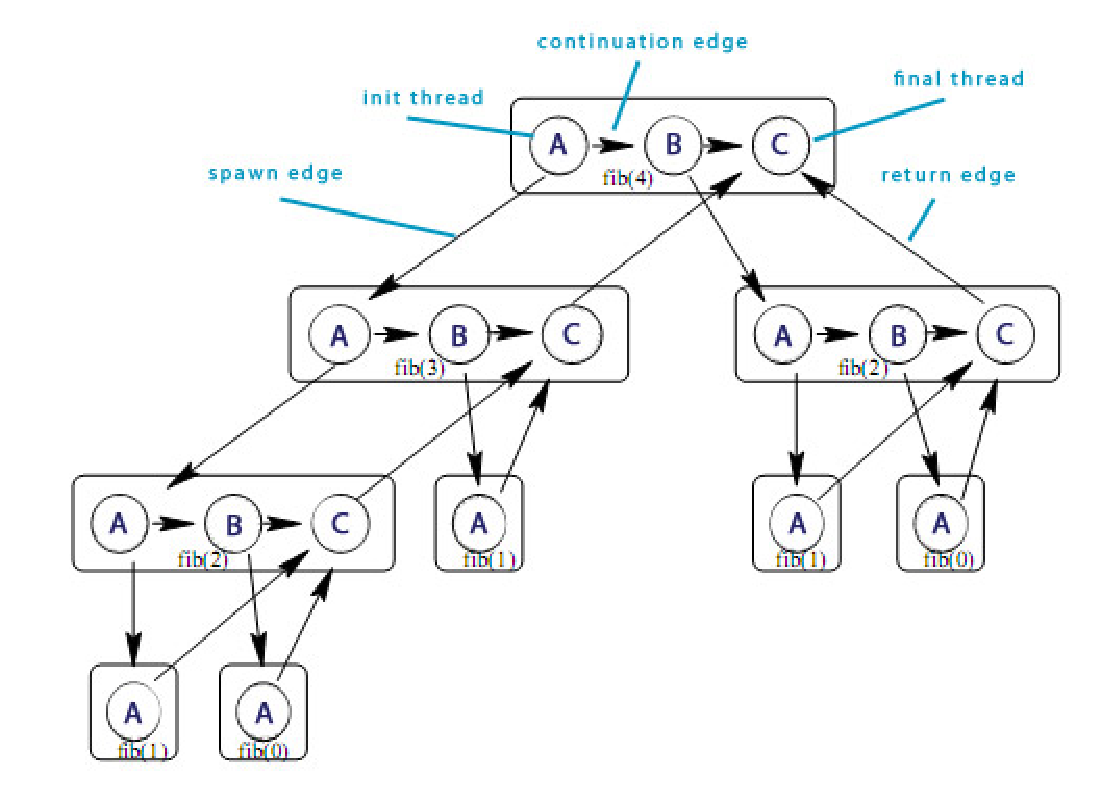
\includegraphics[width=4in]{lecture20/multi-dag.eps}
  \caption{DAG вычисления Fib(4)}
  \label{fig:multi-dag}
\end{figure}

Мы можем рассмотреть выполнение вычисления в контексте динамической
мультипоточности как даг (ориентированный граф без циклов). Будем называть
``потоком'' -- последовательность операций, в которых не содержится связанных с
параллелизмом инструкций (т.е. spawn, sync, return). Потоки образуют множество
вершин дага G.

Выполнение процедуры представляет собой линейную цепочку трэдов, которые
соединяются ``дугами продолжения''. Если трэд $u$ порождает $v$, даг содержит
дугу $(u, v)$, которая назвается ``дугой порождения''. Когда трэд завершает
работу, он соединяется с тем трэдом, который содержит ближайший ``sync'' и эта
дуга называется ``дугой возврата''. Существует стартовый трэд, с которого
начинается вычисления и завершающий трэд, которым оно заканчивается.

\section{Измерение производительности}

Введём две важные характеристики производительности параллельных алгоритмов --
работу и длину критического пути.

Пусть $T_p$ -- это время выполнения алгоритма на $p$ процессорах.

Тогда время выполнения алгоритма на одном процессоре $T_1$ -- это \emph{работа},
а $T_{\infty}$ -- длина критического пути, то есть время выполнения алгоритма,
следуя по самому длинному пути зависимостей в даге. 

В нашем примере $T_1 = 17, T_{\infty} = 8$

Заметим два ограничения снизу, которые накладывают работа и длина критического
пути:

$$
T_p \geqslant T_1 / P
$$

поскольку за один шаг $P$ процессоров могут выполнять как максимум $P$ работы.

$$
T_p \geqslant T_{\infty}
$$

поскольку компьютер с $P$ процессорами не может выполнять больше операций, чем
компьютер с бесконечным количеством процессоров.

Приростом скорости вычисления на $P$ процессорах называется отношение $T_1 /
T_p$, которое показывает насколько быстрее выполняется алгоритм на $P$
процессорах, чем на одном.

Если $T_1/T_p = O(p)$, то мы имеем дело с \emph{линейным приростом}.

Сверхлинейный прирост -- это ещё больше, т.е. $T_1 / T_p > p$, что, однако,
невозможно в рамках нашей модели.

Максимально возможный прирост -- это $T_1 / T_{\infty}$, он называется
``параллелизмом'' задачи и характеризует средний объём работы приходящийся на
каждый шаг вдоль критического пути. Мы будем обозначать его $\bar{P}$

\section{Жадный планировщик}

Программист может управлять значениями работы и длиной критической пути в
процессе кодирования алгоритма, однако непосредственным планированием
распределения задач по потокам занимается планировщик. Существуют весьма сложные
онлайн планировщики, которые хорошо справляются со своей задачей, однако мы их
не будем рассматривать в силу их сложности. Однако практически все идеи можно
продемонстрировать на примере оффлайнового жадного планировщика.

На каждом шаге жадный планировщик пытается запустить на выполнение как можно
большее количество потоков. При использовании компьютера с $P$ процессорами
существует два вида шагов: полный и неполный.

Полный шаг -- это значит, что на начало шага готовы к выполнению $P$ или больше
потоков, таким образом, планировщик просто выбирает любые $P$ потоков и
запускает по одному из них на каждом из $P$ процессоров.

Неполный шаг -- на начало неполного шага имеется меньше $P$ потоков, готовых к
выполнению. Таким образом планировщик может выполнить все из них.

Эта стратегия доказуемо хороша, что  демонстрирует следующая теорема.

\textbf{Теорема Грэма-Брента}. Жадный планировщик выполняет любое многопоточное
вычисление $G$ с работой $T_1$ и длиной критического пути $T_{\infty}$ за время

$$
T_p \leqslant T_1 / P + T_{\infty}
$$

на компьютере с $P$ процессорами.

\textbf{Доказательство}. На каждом шаге производится как максимум $P$ работы.
Таким образом, поскольку на полном шаге все процессоры загружены, то количество
полных шагов может быть ограничено сверху $T_1 / P$, поскольку после выполнения
такого количества шагов вся работа $T_1$ будет сделана и продолжать не имеет
смысла.

Теперь рассмотрим неполный шаг. Пусть $G'$ -- поддаг $G$, который ещё нужно
выполнить. Без потери общности мы можем считать, что все трэды выполняются за
одну единицу времени (чтобы исправить эту проблему -- мы можем заменить более
длительные трэды на цепочку трэдов, которые выполняются за одну единицу
времени). Каждый трэд с входной степенью 0 в $G'$ готов к выполнению, поскольку
все его предшественники уже выполнились. Согласно стратегии жадного планировщика
все эти трэды будут выполнены, поскольку их количество меньше количества
процессоров. Таким образом после выполнения шага -- длина критического пути
уменьшится на единицу (т.к. по сути мы выполняем один уровень дага). Таким
образом количество неполных шагов может быть ограничено длиной критического
пути, т.к. затем уже нечего будет уменьшать.

А поскольку шаг или полный или неполный -- мы можем сложить две оценки сверху и
получить искомое неравенство. $\square$

\textbf{Следствие теоремы}. Жадный планировщик достигает линейного прироста в
скорости, когда $P = O(\bar{P})$

\textbf{Доказательство}. Поскольку $\bar{P} = T_1/T_{\infty}$, то имеем, что $P
= O(T_1/T_{\infty})$ или $T_{\infty} = O(T_1/P)$. Тогда $T(P) \leqslant T_1/P +
T_{\infty} = T_1/P + O(T_1/P) = O(T_1/P)$ что и есть определением линейного
прироста $\square$

\section{Cilk, $\star$Socrates}

Cilk -- это параллельный, многопоточный язык, базирующийся на С, который
разрабатывался в MITе Чарльзом Лейсерсоном и коллегами. Он предоставляет
средства для определения вышеописанных характеристик: работы и длины кратчайшего
пути. В Cilk используется рандомизированный планировщик с ожидаемым временем:
$$
E[T_p] = T_1/P + O(T_{\infty})
$$
и эмпирическим временем:
$$
T_p = T_1/P + T_{\infty}
$$
которое даёт практические идеальный линейный прирост при $P \ll \bar{P}$

Среди многих программ разработанных на Cilk выделяются шахматные прогаммы
$\star$Socrates и Cilkchess, которые выигрывали известные международные
соревнования, сражались с DeepBlue и т.д.

Опишем интересную аномалию, произошедшую при разработке $\star$Socrates.
Изначально разработка производилась на 32-процессорном компьютере в MIT. Однако
соревнование должно было проходить на 512-процессорном компьютере в NCSA. Перед
соревнованием была предложена любопытная оптимизация, которая обеспечивала
значительный прирост на 32-процессорной машине. Однако эта оптимизация не была
принята в финальную версию, поскольку аналитически было определено, что она лишь
замедлит работу на 512-процессорном компьютере. Рассмотрим почему.

\begin{gather*}
  T_{32} = 65 \\
  T'_{32} = 40 \\
  T_1 = 2048 \\
  T_{\infty} = 1 \\
  T_{32} = T_1/P + T_{\infty} = 2048/32 + 1 = 64 + 1 = 65 \\
  T'_1 = 1024 \\
  T'_{\infty} = 8 \\
  T'_{32} = T'_1/P + T_{\infty} = 1024/32 + 8 = 32 + 8 = 40 \\
  T_{512} = 2048/512 + 1 = 5 \\
  T'_{512} = 2048/1024 + 8 = 10
\end{gather*}

Таким образом, на 512-процессорной машине время работы с ``оптимизацией''
замедлилось бы вдвое.

\end{document}
